\chapter[Análisis]{
  \label{chp:analisis}
  ANÁLISIS
}
\thispagestyle{numberingStyle}
\pagestyle{numberingStyle}

En este apartado se explicará, detalladamente, el análisis realizado.

\section{Análisis de requerimientos}

\subsection{Requerimientos funcionales}
A continuación se muestran los requerimientos funcionales del sistema, clasificados en distintas áreas.

\subsubsection*{Acceso a la aplicación}
\begin{itemize}
\setlength\itemsep{1pt}
\item El sistema ofrecerá la posibilidad de que un usuario se registre en la aplicación.
\item El sistema ofrecerá la posibilidad de que el usuario se identifique en el sistema. Los usuarios deben ingresar al sistema con  nombre de usuario y contraseña.
\end{itemize}

\subsubsection*{Cliente Móvil}
\begin{itemize}
\setlength\itemsep{1pt}
\item El sistema ofrecerá la posibilidad de crear nuevas rutas.
\item El usuario podrá consultar las rutas, propias y de otros usuarios, según ciertos criterios de búsqueda.
\item El sistema permitirá a los usuarios autorizados eliminar las rutas propias que deseen.
\item El sistema permitirá a los usuarios autorizados a consultar los detalles de las rutas.
\item Para las rutas, el sistema permitirá:
	\begin{itemize}
	\item Establecer las fechas de inicio y fin.
	\item Consultar, asignar y desasignar a la ruta, los eventos disponibles en esas fechas.
	\item Consultar el itinerario por días.
	\item Modificar la hora de comienzo establecida para cada día.
	\item Consultar, añadir y eliminar lugares de interés a cada día de la ruta.
	\item Editar el modo de viaje a realizar entre diferentes lugares.
	\item Mostrar el itinerario, por días y en total, en el mapa.
	\item Habilitar y deshabilitar el sistema de geolocalización para conocer la ruta hecha en tiempo real.
	\item Consultar y comparar, el itinerario definido con el obtenido a tiempo real.
	\item Editar los permisos de la ruta.
	\end{itemize}
\end{itemize}

\subsubsection*{Cliente Web}
\begin{itemize}
\setlength\itemsep{1pt}
\item El usuario podrá consultar las rutas existentes, propias y de otros usuarios, según ciertos criterios de búsqueda.
\item El sistema permitirá a los usuarios autorizados a consultar los detalles de las rutas.
\item El sistema permitirá a los usuarios autorizados marcar las rutas propias como privadas, con el fin de no compartirlas con los demás usuarios.
\item El sistema solo ofrecerá la posibilidad de consulta sobre los detalles de una ruta, permitiendo ver el itinerario, si tiene datos en tiempo real guardados, etc...
\item El sistema permitirá a los usuarios autorizados eliminar las rutas propias que deseen.
\end{itemize}

\subsubsection*{Cliente Administración Web}
\begin{itemize}
\setlength\itemsep{1pt}
\item El sistema solo permitirá acceso a usuarios con permisos de administración.
\item El sistema permitirá a los usuarios con dichos permisos, dar de alto nuevos usuarios.
\item El sistema permitirá las altas, bajas, modificaciones y consultas de las entidades del sistema.
	\begin{itemize}
	\item El sistema ofrecerá la posibilidad de crear, eliminar, modificar y consultar datos de usuarios.
	\item El sistema ofrecerá la posibilidad de crear, eliminar, modificar y consultar datos de rutas.
	\item El sistema ofrecerá la posibilidad de crear, eliminar, modificar y consultar datos de lugares.
	\item El sistema ofrecerá la posibilidad de crear, eliminar, modificar y consultar datos de categorías.
	\item El sistema ofrecerá la posibilidad de crear, eliminar, modificar y consultar datos de eventos.
	\end{itemize}
\item El sistema permitirá la existencia de usuarios con capacidades para la administración y gestión, exclusivamente, de los eventos. Permitiendo así, sus altas,  bajas, modificaciones y consultas de los mismos en el sistema.
\end{itemize}

\subsubsection*{Seguridad}
\begin{itemize}
\setlength\itemsep{1pt}
\item El sistema ofrecerá la posibilidad de que el usuario modifique sus datos de acceso al sistema.
\item El sistema solo permitirá acciones correctamente autenticadas, exceptuando las de acceso a la aplicación.
\item Los usuarios de la aplicación solo podrán modificar los datos a los que el usuario esté autorizado. Un usuario no podrá modificar la información de los recursos de los que no es propietario.
\item Los intercambios de datos que realice el sistema a través de internet, serán mediante el uso del protocolo encriptado https.
\end{itemize}


\subsection{Requerimientos no funcionales}





\section{Modelo de casos de uso}

\subsection{Actores del sistema}
Analizando los requerimientos funcionales funcionales del sistema, se detectan tres tipos de actores, que demandan una determinada funcionalidad en el sistema. Estos tres actores son, el cliente, el administrador y el gestor de eventos.


\begin{figure}[htbp]
\centering
\vspace*{0.2in}
\includesvg{actores.svg}
\caption{Diagrama casos de uso aplicación móvil.}
\end{figure}


\subsection{Diagrama de casos de uso}
Tras conocer los requerimientos funcionales del sistema y reconocer las necesidades del sistema, se ha optado por diseñar un sistema general compuesto por los diferentes subsistemas del mismo.


\FloatBarrier
\subsubsection*{Diagrama sistema general}
Dicho sistema, estará compuesto por tres grupos de subsistemas: subsistema de acceso, subsistema de administración y subsistema de aplicación.

\begin{figure}[!htbp]
\centering

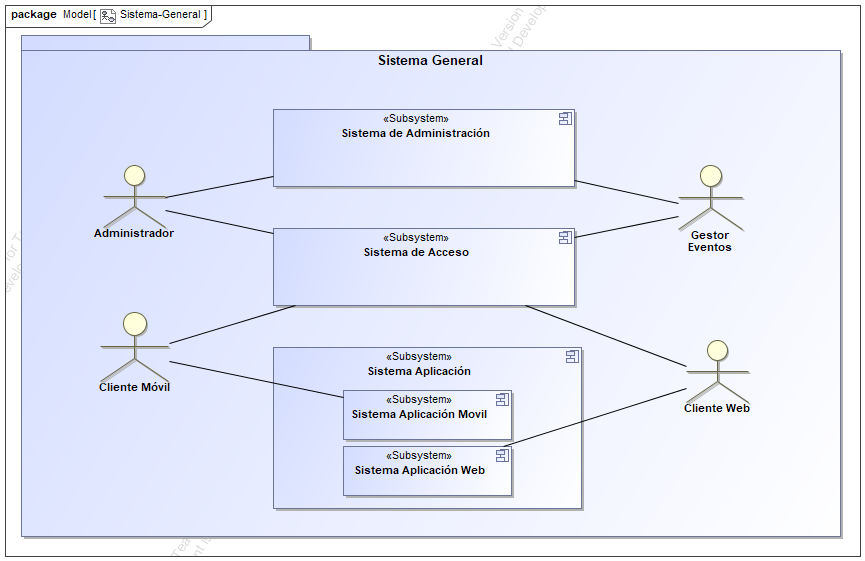
\includegraphics[
   keepaspectratio=true
]{./../Diagrams/uc__Sistema-General.png}
\caption{Diagrama casos de uso - Sistema general.}
\end{figure}


\FloatBarrier
\subsubsection*{Diagrama sistema de acceso}
\begin{figure}[!htbp]
\centering

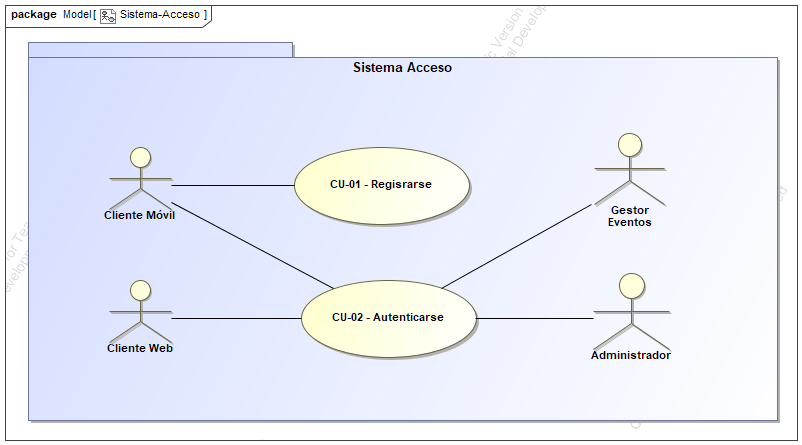
\includegraphics[
   keepaspectratio=true
]{./../Diagrams/uc__Sistema-Acceso.png}
\caption{Diagrama casos de uso - Sistema general.}
\end{figure}


\FloatBarrier
\subsubsection*{Diagrama sistema aplicación móvil}
\begin{figure}[!htbp]
\centering

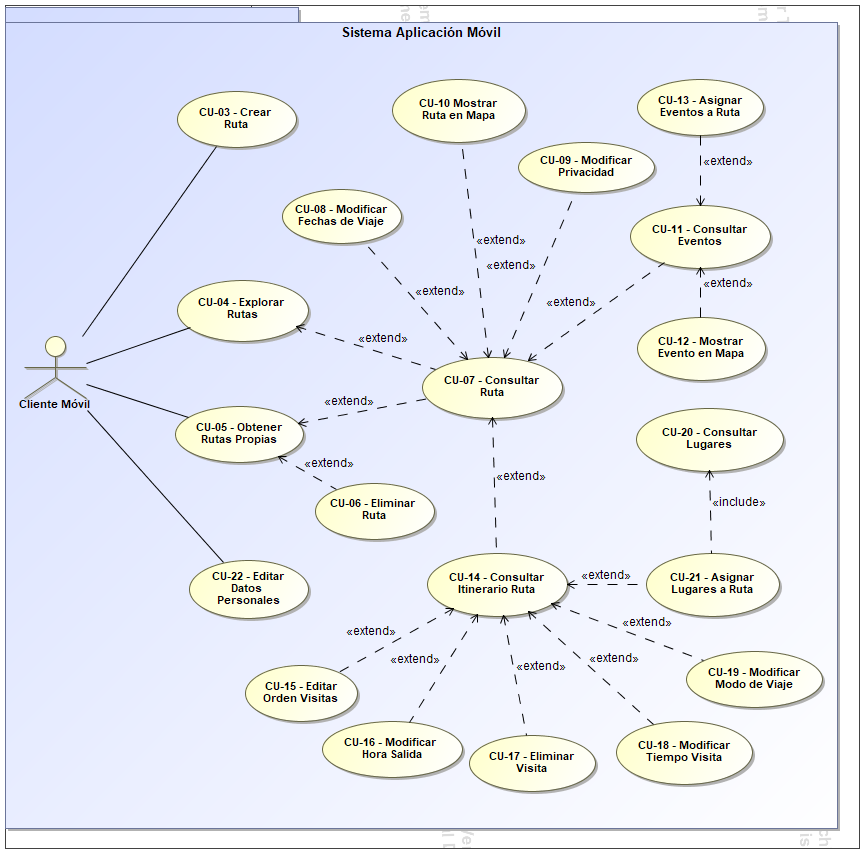
\includegraphics[
   keepaspectratio=true
]{./../Diagrams/Sistema-Aplicacion-Movil.png}
\caption{Diagrama casos de uso - Sistema general.}
\end{figure}


\FloatBarrier
\subsubsection*{Diagrama sistema aplicación web}
\begin{figure}[!htbp]
\centering

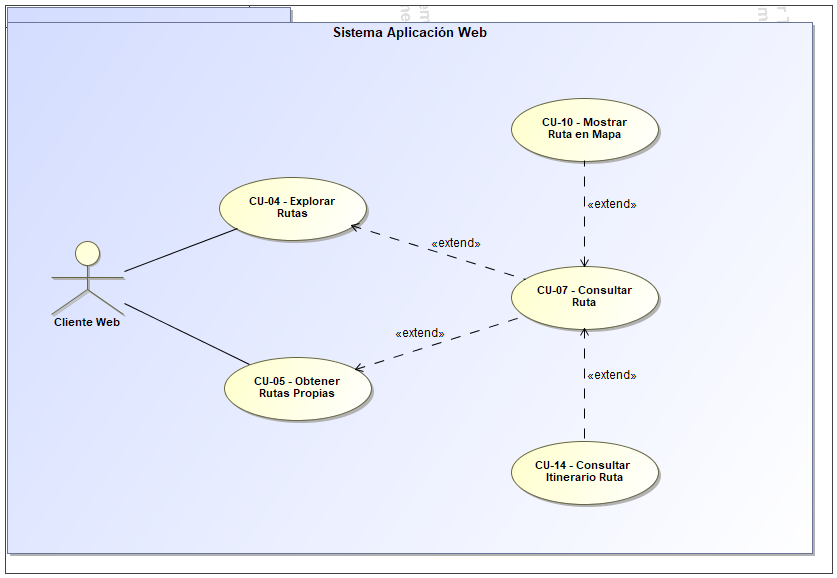
\includegraphics[
   keepaspectratio=true
]{./../Diagrams/Sistema-Aplicacion-Web.png}
\caption{Diagrama casos de uso - Sistema general.}
\end{figure}


\FloatBarrier
\subsubsection*{Diagrama sistema administración}
\begin{figure}[!htbp]
\centering

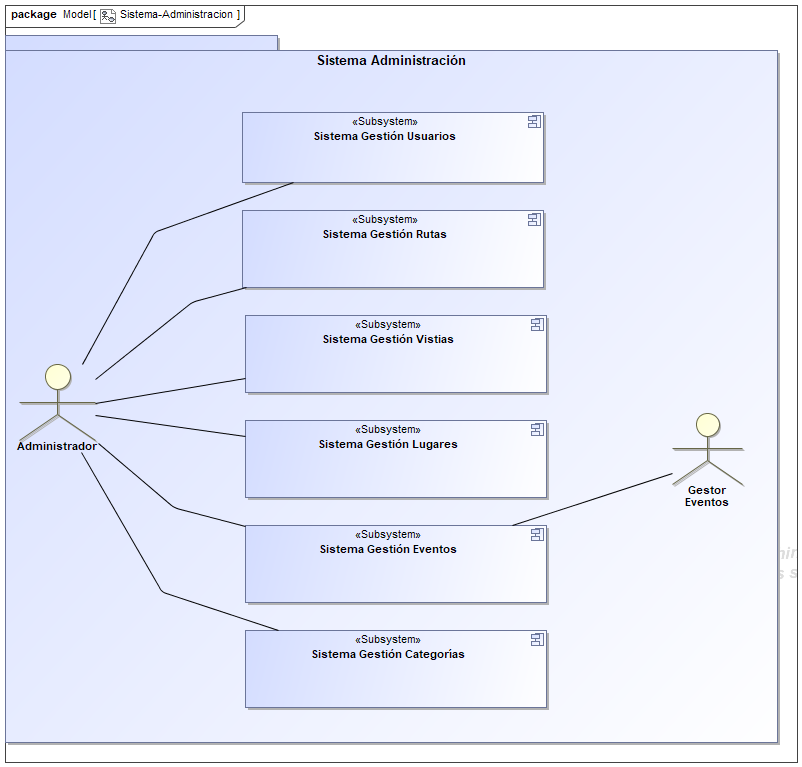
\includegraphics[
   keepaspectratio=true
]{./../Diagrams/Sistema-Administracion.png}
\caption{Diagrama casos de uso - Sistema general.}
\end{figure}


\FloatBarrier
\subsubsection*{Diagrama sistema gestión usuarios}
\begin{figure}[!htbp]
\centering

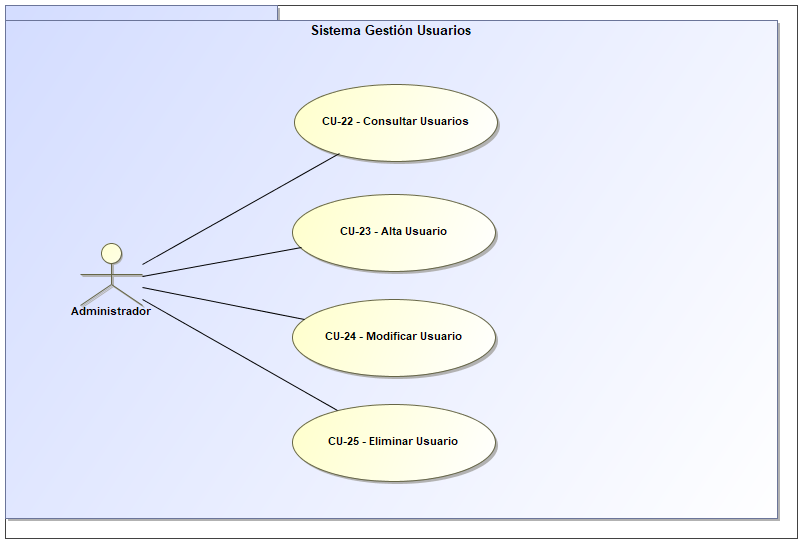
\includegraphics[
   keepaspectratio=true
]{./../Diagrams/Sistema-Gestion-Usuarios.png}
\caption{Diagrama casos de uso - Sistema general.}
\end{figure}


\FloatBarrier
\subsubsection*{Diagrama sistema gestión rutas}
\begin{figure}[!htbp]
\centering

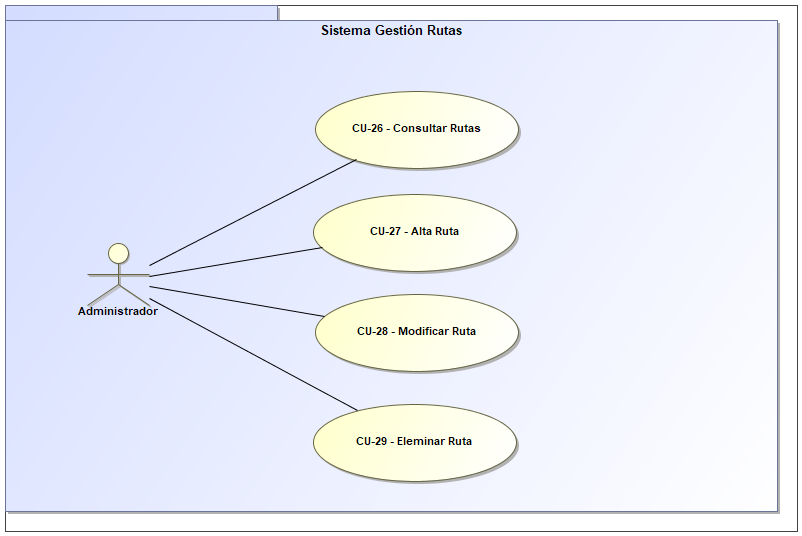
\includegraphics[
   keepaspectratio=true
]{./../Diagrams/Sistema-Gestion-Rutas.png}
\caption{Diagrama casos de uso - Sistema general.}
\end{figure}


\FloatBarrier
\subsubsection*{Diagrama sistema gestión lugares}
\begin{figure}[!htbp]
\centering

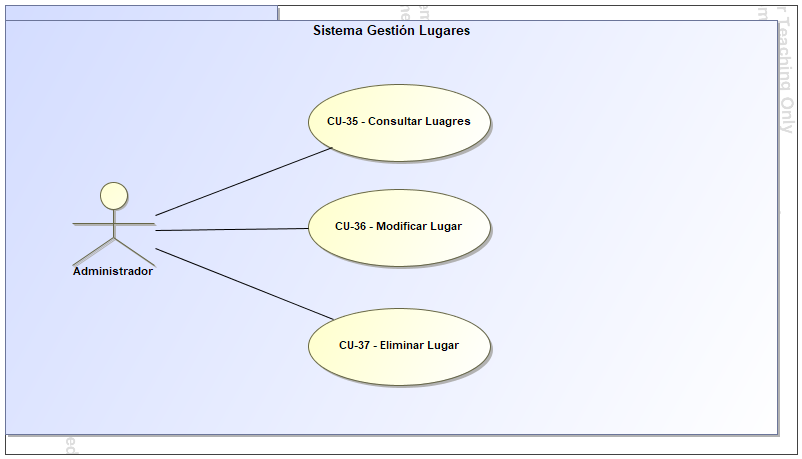
\includegraphics[
   keepaspectratio=true
]{./../Diagrams/Sistema-Gestion-Lugares.png}
\caption{Diagrama casos de uso - Sistema general.}
\end{figure}


\FloatBarrier
\subsubsection*{Diagrama sistema gestión eventos}
\begin{figure}[!htbp]
\centering

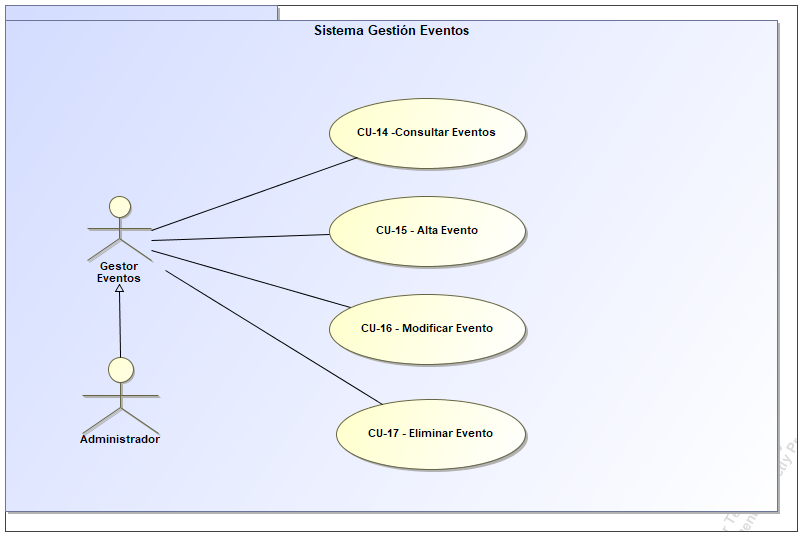
\includegraphics[
   keepaspectratio=true
]{./../Diagrams/Sistema-Gestion-Eventos.png}
\caption{Diagrama casos de uso - Sistema general.}
\end{figure}


\FloatBarrier
\subsubsection*{Diagrama sistema gestión categorías}
\begin{figure}[!htbp]
\centering

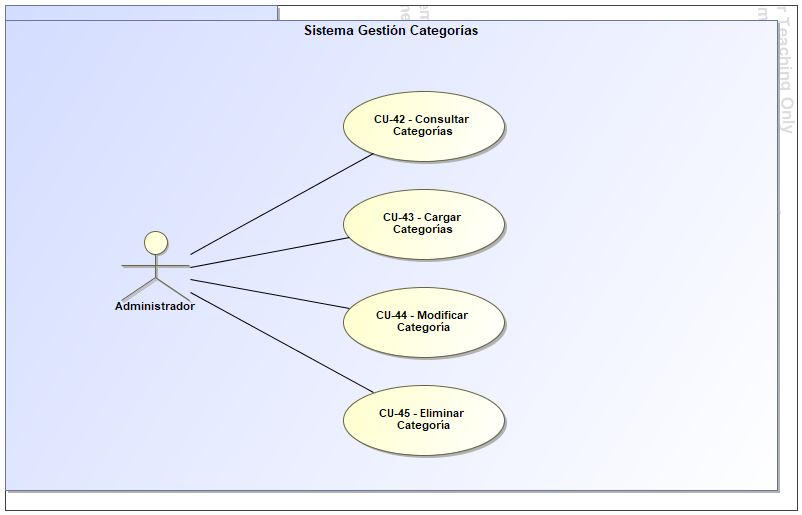
\includegraphics[
   keepaspectratio=true
]{./../Diagrams/Sistema-Gestion-Categorias.png}
\caption{Diagrama casos de uso - Sistema general.}
\end{figure}



\newpage
\subsection{Especificación casos de uso}


\newpage
\subsubsection*{Caso de uso: Autenticarse}
\begin{longtable}{| p{4cm} | p{10cm} |}
\endfirsthead
\multicolumn{2}{c}{\textit{Continúa de la página anterior}}\\[12pt]
\hline
\endhead
\hline
\multicolumn{2}{c}{\textit{Continúa en la siguiente página}} \\
\endfoot
\hline
\caption{Caso de Uso: Autenticarse}\label{fig:1}\\
\endlastfoot


\hline
\multicolumn{2}{|c|}{\textbf{CU$<$01$>$ - Autenticarse}} \\

\hline
\textbf{Descripción} &
El usuario se identifica introduciendo las credenciales de acceso en el sistema \\

\hline
\textbf{Actores} &
Cliente Móvil\newline
Cliente Web\newline
Administrador\newline
Moderador\\

\hline
\textbf{Precondiciones} &
\\

\hline
\textbf{Secuencia Normal} &\mbox{}\par\vspace{-\baselineskip}
\begin{enumerate}[leftmargin=0.7cm, topsep=0.1cm]
\item El usuario introduce sus credenciales en la ventana de login. 
\item El usuario pulsa el botón de \textit{Acceder}.
\item El sistema valida las credenciales.
\item El usuario accede a la aplicación.
\end{enumerate}\\

\hline
\textbf{Excepciones} &\mbox{}\par\vspace{-\baselineskip}
\begin{enumerate}[leftmargin=0.9cm, topsep=0.1cm]
\item[3.] Los datos introducidos no son correctos.
	\begin{itemize}
	\item[1.] El sistema muestra un mensaje de error y regresa al \textit{Paso 1}.
	\end{itemize}

\end{enumerate}\\

\hline
\textbf{Postcondiciones} & 
El usuario queda autenticado en el sistema\\
\hline
\end{longtable}




\newpage
\subsubsection*{Caso de uso: Registrarse}
\begin{longtable}{| p{4cm} | p{10cm} |}
\endfirsthead
\multicolumn{2}{c}{\textit{Continúa de la página anterior}}\\[12pt]
\hline
\endhead
\hline
\multicolumn{2}{c}{\textit{Continúa en la siguiente página}} \\
\endfoot
\hline
\caption{Caso de Uso: Registrarse}\label{fig:1}\\
\endlastfoot


\hline
\multicolumn{2}{|c|}{\textbf{CU$<$02$>$ - Registrarse}} \\

\hline
\textbf{Descripción} &
El usuario introduce los datos para darse de alta en la aplicación. \\

\hline
\textbf{Actores} &
Cliente Móvil\\


\hline
\textbf{Precondiciones} &
N/A\\

\hline
\textbf{Secuencia Normal} &\mbox{}\par\vspace{-\baselineskip}
\begin{enumerate}[leftmargin=0.7cm, topsep=0.1cm]
\item El usuario selecciona la opción de registro.
\item El sistema muestra un formulario indicando los campos necesarios para realizar el registro.
\item El usuario rellena los campos y pulsa el botón de \textit{Registrarse}.
\item El sistema valida los datos introducidos por el usuario.
\item El usuario accede a la aplicación.
\end{enumerate}\\

\hline
\textbf{Excepciones} &\mbox{}\par\vspace{-\baselineskip}
\begin{enumerate}[leftmargin=0.9cm, topsep=0.1cm]
\item[3.] El usuario pulsa el botón de \textit{Cancelar}.
	\begin{itemize}
	\item[1.] El sistema cancela el registro y redirige al usuario a la pantalla de login.
	\end{itemize}
\item[4.] Los datos introducidos por el usuario no son válidos.
	\begin{itemize}
	\item[1.] El sistema muestra un mensaje de error y regresa al \textit{Paso 2}.
	\end{itemize}
\end{enumerate}\\

\hline
\textbf{Postcondiciones} & 
El usuario queda registrado y autenticado en el sistema\\
\hline
\end{longtable}




\newpage
\subsubsection*{Caso de uso: Crear ruta}
\begin{longtable}{| p{4cm} | p{10cm} |}
\endfirsthead
\multicolumn{2}{c}{\textit{Continúa de la página anterior}}\\[12pt]
\hline
\endhead
\hline
\multicolumn{2}{c}{\textit{Continúa en la siguiente página}} \\
\endfoot
\hline
\caption{Caso de Uso: Crear ruta}\label{fig:1}\\
\endlastfoot


\hline
\multicolumn{2}{|c|}{\textbf{CU$<$03$>$ - Crear Ruta}} \\

\hline
\textbf{Descripción} &
El usuario crea una ruta para una ciudad o lugar especificado. \\

\hline
\textbf{Actores} &
Cliente Móvil\\

\hline
\textbf{Precondiciones} &
El usuario está autenticado en la aplicación\\

\hline
\textbf{Secuencia Normal} &\mbox{}\par\vspace{-\baselineskip}
\begin{enumerate}[leftmargin=0.7cm, topsep=0.1cm]
\item El usuario selecciona la opción de crear una nueva ruta.
\item El sistema muestra buscador para que el usuario indique en qué ciudad o lugar desea crear dicha ruta.
\item El usuario rellena el buscador.
\item El sistema ayuda al usuario autocompletando con los datos de diferentes ciudades y lugares.
\item El usuario selecciona el lugar en la lista de autocompletado ofrecida por el sistema.
\item El sistema muestra un mapa indicando la ubicación del lugar seleccionado y permite al usuario completar el proceso de creación.
\item El usuario pulsa el botón para crear la ruta.
\end{enumerate}\\

\hline
\textbf{Excepciones} &\mbox{}\par\vspace{-\baselineskip}
\\

\hline
\textbf{Postcondiciones} & 
La ruta queda registrada en el sistema\\
\hline
\end{longtable}




\newpage
\subsubsection*{Caso de uso: Explorar rutas}
\begin{longtable}{| p{4cm} | p{10cm} |}
\endfirsthead
\multicolumn{2}{c}{\textit{Continúa de la página anterior}}\\[12pt]
\hline
\endhead
\hline
\multicolumn{2}{c}{\textit{Continúa en la siguiente página}} \\
\endfoot
\hline
\caption{Caso de Uso: Explorar rutas}\label{fig:1}\\
\endlastfoot


\hline
\multicolumn{2}{|c|}{\textbf{CU$<$04$>$ - Explorar Rutas}} \\

\hline
\textbf{Descripción} &
El usuario explora las diferentes rutas creadas por los demás usuarios.\\

\hline
\textbf{Actores} &
Cliente Móvil\newline
Cliente Web\\

\hline
\textbf{Precondiciones} &
El usuario está autenticado en la aplicación\\

\hline
\textbf{Secuencia Normal} &\mbox{}\par\vspace{-\baselineskip}
\begin{enumerate}[leftmargin=0.7cm, topsep=0.1cm]
\item El usuario selecciona la opción de explorar rutas.
\item El sistema muestra las diferentes rutas que hay en el sistema.
\end{enumerate}\\

\hline
\textbf{Excepciones} &\mbox{}\par\vspace{-\baselineskip}
\\

\hline
\textbf{Postcondiciones} & 
\\
\hline
\end{longtable}



\newpage
\subsubsection*{Caso de uso: Obtener rutas propias}
\begin{longtable}{| p{4cm} | p{10cm} |}
\endfirsthead
\multicolumn{2}{c}{\textit{Continúa de la página anterior}}\\[12pt]
\hline
\endhead
\hline
\multicolumn{2}{c}{\textit{Continúa en la siguiente página}} \\
\endfoot
\hline
\caption{Caso de Uso: Obtener Rutas propias}\label{fig:1}\\
\endlastfoot


\hline
\multicolumn{2}{|c|}{\textbf{CU$<$05$>$ - Obtener Rutas Propias}} \\

\hline
\textbf{Descripción} &
El usuario obtiene las rutas creadas por él.\\

\hline
\textbf{Actores} &
Cliente Móvil\newline
Cliente Web\\

\hline
\textbf{Precondiciones} &
El usuario está autenticado en la aplicación\\

\hline
\textbf{Secuencia Normal} &\mbox{}\par\vspace{-\baselineskip}
\begin{enumerate}[leftmargin=0.7cm, topsep=0.1cm]
\item El usuario selecciona la opción de obtener rutas propias.
\item El sistema muestra las rutas que tiene almacenadas en el sistema y.
\item El sistema clasifica las rutas del usuario en función de su progreso; las que aún no empezaron, las que están en curso y las que ya se realizaron.
\item El usuario selecciona una de las posibilidades ofrecidas por el sistema.
\item El sistema filtra las rutas del usuario según lo solicitado.
\end{enumerate}\\

\hline
\textbf{Excepciones} &\mbox{}\par\vspace{-\baselineskip}
\\

\hline
\textbf{Postcondiciones} & 
\\
\hline
\end{longtable}




\newpage
\subsubsection*{Caso de uso: Consultar ruta}
\begin{longtable}{| p{4cm} | p{10cm} |}
\endfirsthead
\multicolumn{2}{c}{\textit{Continúa de la página anterior}}\\[12pt]
\hline
\endhead
\hline
\multicolumn{2}{c}{\textit{Continúa en la siguiente página}} \\
\endfoot
\hline
\caption{Caso de Uso: Consultar ruta}\label{fig:1}\\
\endlastfoot


\hline
\multicolumn{2}{|c|}{\textbf{CU$<$06$>$ - Consultar Ruta}} \\

\hline
\textbf{Descripción} &
El usuario obtiene la información detallada de una ruta concreta.\\

\hline
\textbf{Actores} &
Cliente Móvil\newline
Cliente Web\\

\hline
\textbf{Precondiciones} &
\\

\hline
\textbf{Secuencia Normal} &\mbox{}\par\vspace{-\baselineskip}
\begin{enumerate}[leftmargin=0.7cm, topsep=0.1cm]
\item El usuario selecciona una ruta concreta.
\item El sistema obtiene los datos de la ruta.
\item El sistema muestra un panel con los datos detallados de la ruta.
\end{enumerate}\\

\hline
\textbf{Excepciones} &\mbox{}\par\vspace{-\baselineskip}
\begin{enumerate}[leftmargin=0.9cm, topsep=0.1cm]
\item[3.] El usuario pulsa el botón de \textit{Atrás}.
	\begin{itemize}
	\item[1.] El sistema devuelve al usuario a la vista anterior.
	\end{itemize}
\end{enumerate}
\\

\hline
\textbf{Postcondiciones} & 
\\
\hline
\end{longtable}



\newpage
\subsubsection*{Caso de uso: Modificar fechas de viaje}
\begin{longtable}{| p{4cm} | p{10cm} |}
\endfirsthead
\multicolumn{2}{c}{\textit{Continúa de la página anterior}}\\[12pt]
\hline
\endhead
\hline
\multicolumn{2}{c}{\textit{Continúa en la siguiente página}} \\
\endfoot
\hline
\caption{Caso de Uso: Modificar fechas de viaje}\label{fig:1}\\
\endlastfoot


\hline
\multicolumn{2}{|c|}{\textbf{CU$<$07$>$ - Modificar Fechas de Viaje}} \\

\hline
\textbf{Descripción} &
El usuario selecciona las fechas en las que se realizará la ruta que está planificando.\\

\hline
\textbf{Actores} &
Cliente Móvil\\

\hline
\textbf{Precondiciones} &
\\

\hline
\textbf{Secuencia Normal} &\mbox{}\par\vspace{-\baselineskip}
\begin{enumerate}[leftmargin=0.7cm, topsep=0.1cm]
\item El usuario selecciona la opción de \textit{Seleccionar Fechas}.
\item El sistema muestra una pantalla con las fechas del calendario.
\item El usuario selecciona la fecha de inicio y fin y pulsa el botón de \textit{Aceptar}.
\item El sistema modifica las fechas de la ruta.
\end{enumerate}\\

\hline
\textbf{Excepciones} &\mbox{}\par\vspace{-\baselineskip}
\begin{enumerate}[leftmargin=0.9cm, topsep=0.1cm]
\item[3.] El usuario pulsa el botón de \textit{Cancelar}.
	\begin{itemize}
	\item[1.] El sistema cancela la modificación de las fechas y cierra la pantalla.
	\end{itemize}
\end{enumerate}
\\

\hline
\textbf{Postcondiciones} & 
Las fechas de la ruta quedan actualizadas en el sistema.\\
\hline
\end{longtable}



\newpage
\subsubsection*{Caso de uso: Modificar privacidad}
\begin{longtable}{| p{4cm} | p{10cm} |}
\endfirsthead
\multicolumn{2}{c}{\textit{Continúa de la página anterior}}\\[12pt]
\hline
\endhead
\hline
\multicolumn{2}{c}{\textit{Continúa en la siguiente página}} \\
\endfoot
\hline
\caption{Caso de Uso: Modificar privacidad}\label{fig:1}\\
\endlastfoot


\hline
\multicolumn{2}{|c|}{\textbf{CU$<$08$>$ - Modificar Privacidad}} \\

\hline
\textbf{Descripción} &
El usuario puede alternar la privacidad de cada una de sus rutas permitiendo que sean visible para todos o solo para él.\\

\hline
\textbf{Actores} &
Cliente Móvil\\

\hline
\textbf{Precondiciones} &
\\

\hline
\textbf{Secuencia Normal} &\mbox{}\par\vspace{-\baselineskip}
\begin{enumerate}[leftmargin=0.7cm, topsep=0.1cm]
\item El usuario selecciona la opción de \textit{Detalles de la Ruta}.
\item El sistema muestra una pantalla con los detalles de la ruta.
\item El sistema incluye un botón que permite alternar entre los estados de privacidad.
\item El usuario pulsa el botón.
\item El sistema cambia el valor del botón y actualiza el nuevo valor de privacidad.
\end{enumerate}\\

\hline
\textbf{Excepciones} &\mbox{}\par\vspace{-\baselineskip}
\begin{enumerate}[leftmargin=0.9cm, topsep=0.1cm]
\item[4.] El usuario pulsa el botón de \textit{Atrás}.
	\begin{itemize}
	\item[1.] El sistema retorna a la pantalla anterior.
	\end{itemize}
\end{enumerate}
\\

\hline
\textbf{Postcondiciones} & 
La privacidad de la ruta queda actualizada.\\
\hline
\end{longtable}



\newpage
\subsubsection*{Caso de uso: Mostrar ruta en mapa}
\begin{longtable}{| p{4cm} | p{10cm} |}
\endfirsthead
\multicolumn{2}{c}{\textit{Continúa de la página anterior}}\\[12pt]
\hline
\endhead
\hline
\multicolumn{2}{c}{\textit{Continúa en la siguiente página}} \\
\endfoot
\hline
\caption{Caso de Uso: Mostrar Ruta en Mapa}\label{fig:1}\\
\endlastfoot


\hline
\multicolumn{2}{|c|}{\textbf{CU$<$09$>$ - Mostrar Ruta en Mapa}} \\

\hline
\textbf{Descripción} &
El usuario puede mostrar la información de la ruta en el mapa.\\

\hline
\textbf{Actores} &
Cliente Móvil\newline
Cliente Web\\

\hline
\textbf{Precondiciones} &
\\

\hline
\textbf{Secuencia Normal} &\mbox{}\par\vspace{-\baselineskip}
\begin{enumerate}[leftmargin=0.7cm, topsep=0.1cm]
\item El usuario selecciona la opción de \textit{Mostrar Ruta en Mapa}.
\item El sistema muestra un mapa con las marcas de los lugares asignados a la ruta en un día concreto de la ruta.
\item Si la ruta ya ha transcurrido en el tiempo y tiene información de su ejecución en tiempo real.
	\begin{itemize}
	\item[1.] El sistema incorpora al mapa la ruta real realizada por el usuario permitiendo compararla con la ruta planificada.
	\end{itemize}
\item El usuario puede cambiar entre los días haciendo click sobre ellos.
\end{enumerate}\\

\hline
\textbf{Excepciones} &\mbox{}\par\vspace{-\baselineskip}
\begin{enumerate}[leftmargin=0.9cm, topsep=0.1cm]
\item[3.] El usuario pulsa el botón de \textit{Atrás}.
	\begin{itemize}
	\item[1.] El sistema retorna a la pantalla anterior.
	\end{itemize}
\end{enumerate}
\\

\hline
\textbf{Postcondiciones} & \\
\hline
\end{longtable}



\newpage
\subsubsection*{Caso de uso: Consultar eventos}
\begin{longtable}{| p{4cm} | p{10cm} |}
\endfirsthead
\multicolumn{2}{c}{\textit{Continúa de la página anterior}}\\[12pt]
\hline
\endhead
\hline
\multicolumn{2}{c}{\textit{Continúa en la siguiente página}} \\
\endfoot
\hline
\caption{Caso de Uso: Cosnultar eventos}\label{fig:1}\\
\endlastfoot


\hline
\multicolumn{2}{|c|}{\textbf{CU$<$10$>$ - Consultar Eventos}} \\

\hline
\textbf{Descripción} &
El usuario obtiene los eventos dados de alta en el sistema\\

\hline
\textbf{Actores} &
Cliente Móvil\\

\hline
\textbf{Precondiciones} &
\\

\hline
\textbf{Secuencia Normal} &\mbox{}\par\vspace{-\baselineskip}
\begin{enumerate}[leftmargin=0.7cm, topsep=0.1cm]
\item El usuario selecciona la opción de \textit{Consultar Eventos}.
\item El sistema muestra una pantalla con las opciones: \textit{En el viaje} y \textit{Próximos}.
\item Si el usuario selecciona \textit{En el viaje}.
	\begin{itemize}
	\item[1.] El sistema muestra los eventos que coinciden durante las fechas de viaje del usuario.
	\end{itemize}
\item Si el usuario selecciona \textit{Próximos}.
	\begin{itemize}
	\item[1.] El sistema muestra los eventos futuros a las fechas de viaje del usuario.
	\end{itemize}
\end{enumerate}\\

\hline
\textbf{Excepciones} &\mbox{}\par\vspace{-\baselineskip}
\begin{enumerate}[leftmargin=0.9cm, topsep=0.1cm]
\item[3-4.] El usuario pulsa el botón de \textit{Atrás}.
	\begin{itemize}
	\item[1.] El sistema retorna a la pantalla anterior.
	\end{itemize}
\end{enumerate}
\\

\hline
\textbf{Postcondiciones} & \\
\hline
\end{longtable}



\newpage
\subsubsection*{Caso de uso: Mostrar evento en mapa }
\begin{longtable}{| p{4cm} | p{10cm} |}
\endfirsthead
\multicolumn{2}{c}{\textit{Continúa de la página anterior}}\\[12pt]
\hline
\endhead
\hline
\multicolumn{2}{c}{\textit{Continúa en la siguiente página}} \\
\endfoot
\hline
\caption{Caso de Uso: Mostrar Evento en Mapa}\label{fig:1}\\
\endlastfoot


\hline
\multicolumn{2}{|c|}{\textbf{CU$<$11$>$ - Mostrar Evento en Mapa}} \\

\hline
\textbf{Descripción} &
Muestra un evento concreto en el mapa.\\

\hline
\textbf{Actores} &
Cliente Móvil\\

\hline
\textbf{Precondiciones} &
\\

\hline
\textbf{Secuencia Normal} &\mbox{}\par\vspace{-\baselineskip}
\begin{enumerate}[leftmargin=0.7cm, topsep=0.1cm]
\item El usuario selecciona la opción de \textit{Mostrar Evento en Mapa}.
\item El sistema muestra un mapa indicando la ubicación del evento.
\item El sistema incluye la ubicación de los lugares asignados al día de la ruta que transcurre el mismo día del evento, permitiendo ubicar el evento en función de la ruta ya creada.
\end{enumerate}
\\
\hline
\textbf{Excepciones} &\mbox{}\par\vspace{-\baselineskip}
\begin{enumerate}[leftmargin=0.9cm, topsep=0.1cm]
\item[2-3.] El usuario pulsa el botón de \textit{Atrás}.
	\begin{itemize}
	\item[1.] El sistema retorna a la pantalla anterior.
	\end{itemize}
\end{enumerate}
\\

\hline
\textbf{Postcondiciones} & \\
\hline
\end{longtable}



\newpage
\subsubsection*{Caso de uso: Asignar eventos a ruta }
\begin{longtable}{| p{4cm} | p{10cm} |}
\endfirsthead
\multicolumn{2}{c}{\textit{Continúa de la página anterior}}\\[12pt]
\hline
\endhead
\hline
\multicolumn{2}{c}{\textit{Continúa en la siguiente página}} \\
\endfoot
\hline
\caption{Caso de Uso: Asignar evento a ruta}\label{fig:1}\\
\endlastfoot


\hline
\multicolumn{2}{|c|}{\textbf{CU$<$12$>$ - Asignar Evento a ruta}} \\

\hline
\textbf{Descripción} &
Permite incorporar o eliminar eventos a la ruta.\\

\hline
\textbf{Actores} &
Cliente Móvil\\

\hline
\textbf{Precondiciones} &
\\

\hline
\textbf{Secuencia Normal} &\mbox{}\par\vspace{-\baselineskip}
\begin{enumerate}[leftmargin=0.7cm, topsep=0.1cm]
\item Si el evento no está asignado a la ruta.
	\begin{itemize}
	\item[1.] El sistema muestra un botón para añadir dicho evento.
	 en la ruta del usuario.
	\end{itemize}
\item Si el evento ya está asignado a la ruta.
	\begin{itemize}
	\item[1.] El sistema muestra un botón para eliminar dicho evento de la ruta.
	\end{itemize}
\item El usuario clicka el botón correspondiente.
\item El sistema muestra un una ventana de confirmación.
\item El usuario pulsa en \textit{Aceptar}
\item El sistema incorpora o elimina el evento al día correspondiente.
\end{enumerate}


\\
\hline
\textbf{Excepciones} &\mbox{}\par\vspace{-\baselineskip}
\begin{enumerate}[leftmargin=0.9cm, topsep=0.1cm]
\item[2.] El usuario pulsa el botón de \textit{Atrás}.
	\begin{itemize}
	\item[1.] El sistema retorna a la pantalla anterior.
	\end{itemize}
\item[5.] El usuario pulso en \textit{Cancelar} en la ventana de confirmación.
	\begin{itemize}
	\item[1.] El sistema cancela la confirmación y retorna al \textit{Paso 1}
	\end{itemize}
\item[6.] El sistema no puede realizar la acción solicitada.
	\begin{itemize}
	\item[1.] El sistema cancela la acción y muestra un error al usuario.
	\end{itemize}
\end{enumerate}
\\

\hline
\textbf{Postcondiciones} & \\
\hline
\end{longtable}



\newpage
\subsubsection*{Caso de uso: Consultar itinerario ruta }
\begin{longtable}{| p{4cm} | p{10cm} |}
\endfirsthead
\multicolumn{2}{c}{\textit{Continúa de la página anterior}}\\[12pt]
\hline
\endhead
\hline
\multicolumn{2}{c}{\textit{Continúa en la siguiente página}} \\
\endfoot
\hline
\caption{Caso de Uso: Consultar itinerario ruta}\label{fig:1}\\
\endlastfoot


\hline
\multicolumn{2}{|c|}{\textbf{CU$<$13$>$ - Consultar Itinerario Ruta}} \\

\hline
\textbf{Descripción} &
Obtiene la información de la ruta desglosada por los días que la componen.\\

\hline
\textbf{Actores} &
Cliente Móvil\newline
Cliente Web\\

\hline
\textbf{Precondiciones} &
La ruta tiene unas fechas de viaje asignadas.\\

\hline
\textbf{Secuencia Normal} &\mbox{}\par\vspace{-\baselineskip}
\begin{enumerate}[leftmargin=0.7cm, topsep=0.1cm]
\item El usuario selecciona la opción \textit{Itinerario}.
\item El sistema muestra en la parte superior un selector con los días y en la inferior la información correspondiente a cada día. Para cada día, el sistema muestra:
	\begin{itemize}
	\item [1.] El conjunto de visitas a lugares y/o eventos asignadas por el usuario.
	\item [2.] La hora de comienzo de la ruta para el día determinado.
	\item [3.] La hora de llegada, estimada, a cada visita.
	\item [4.] El tiempo asignado, como parada, en cada visita.
	\item [5.] La hora de salida, estimada, para cada visita.
	\item [6.] El modo de viaje, junto a su duración y distancia, entre cada visita.
	\item [7.] Un botón para eliminar la visita.
	\end{itemize}
\item El usuario cambia de día haciendo uso del selector.
\end{enumerate}


\\
\hline
\textbf{Excepciones} &\mbox{}\par\vspace{-\baselineskip}
\begin{enumerate}[leftmargin=0.9cm, topsep=0.1cm]
\item[2-3.] El usuario pulsa el botón de \textit{Atrás}.
	\begin{itemize}
	\item[1.] El sistema retorna a la pantalla anterior.
	\end{itemize}
\end{enumerate}
\\

\hline
\textbf{Postcondiciones} & \\
\hline
\end{longtable}



\newpage
\subsubsection*{Caso de uso: Editar orden visitas }
\begin{longtable}{| p{4cm} | p{10cm} |}
\endfirsthead
\multicolumn{2}{c}{\textit{Continúa de la página anterior}}\\[12pt]
\hline
\endhead
\hline
\multicolumn{2}{c}{\textit{Continúa en la siguiente página}} \\
\endfoot
\hline
\caption{Caso de Uso: Editar orden visitas}\label{fig:1}\\
\endlastfoot


\hline
\multicolumn{2}{|c|}{\textbf{CU$<$14$>$ - Editar Orden Visitas}} \\

\hline
\textbf{Descripción} &
Modifica el orden de las visitas establecidas para un día.\\

\hline
\textbf{Actores} &
Cliente Móvil\\

\hline
\textbf{Precondiciones} &
\\

\hline
\textbf{Secuencia Normal} &\mbox{}\par\vspace{-\baselineskip}
\begin{enumerate}[leftmargin=0.7cm, topsep=0.1cm]
\item El usuario selecciona la opción \textit{Habilitar Edición}.
\item El sistema muestra la vista de edición para las visitas.
\item El usuario modifica el orden de las visitas.
\item El sistema actualiza el orden establecido y recalcula las distancias y tiempos de viaje para el nuevo orden de las visitas.
\item El usuario selecciona \textit{Terminar Edición}.
\item El sistema vuelve a la vista normal.
\end{enumerate}


\\
\hline
\textbf{Excepciones} &\mbox{}\par\vspace{-\baselineskip}
\begin{enumerate}[leftmargin=0.9cm, topsep=0.1cm]
\item[3-5.] El usuario pulsa el botón de \textit{Atrás}.
	\begin{itemize}
	\item[1.] El sistema retorna a la pantalla anterior.
	\end{itemize}
\end{enumerate}
\\

\hline
\textbf{Postcondiciones} & \\
\hline
\end{longtable}



\newpage
\subsubsection*{Caso de uso: Modificar hora de salida }
\begin{longtable}{| p{4cm} | p{10cm} |}
\endfirsthead
\multicolumn{2}{c}{\textit{Continúa de la página anterior}}\\[12pt]
\hline
\endhead
\hline
\multicolumn{2}{c}{\textit{Continúa en la siguiente página}} \\
\endfoot
\hline
\caption{Caso de Uso: Modificar hora de salida}\label{fig:1}\\
\endlastfoot


\hline
\multicolumn{2}{|c|}{\textbf{CU$<$15$>$ - Modificar Hora de Salida}} \\

\hline
\textbf{Descripción} &
Modifica la hora de salida para un día concreto de la ruta.\\

\hline
\textbf{Actores} &
Cliente Móvil\\

\hline
\textbf{Precondiciones} &
\\

\hline
\textbf{Secuencia Normal} &\mbox{}\par\vspace{-\baselineskip}
\begin{enumerate}[leftmargin=0.7cm, topsep=0.1cm]
\item El usuario selecciona la opción \textit{Modificar hora de salida}.
\item El sistema muestra un formulario para indicar la hora deseada.
\item El usuario selecciona la hora en el formulario y pulsa en \textit{Confirmar}.
\item El sistema valida la hora y la actualiza.
\end{enumerate}


\\
\hline
\textbf{Excepciones} &\mbox{}\par\vspace{-\baselineskip}
\begin{enumerate}[leftmargin=0.9cm, topsep=0.1cm]
\item[3.] El usuario pulsa el botón de \textit{Cancelar}.
	\begin{itemize}
	\item[1.] El sistema deshecha el formulario y cancela la acción.
	\end{itemize}
\item[4.] El sistema no puede realizar la acción solicitada.
	\begin{itemize}
	\item[1.] El sistema cancela la acción y muestra un error al usuario.
	\end{itemize}
\end{enumerate}
\\

\hline
\textbf{Postcondiciones} & 
La hora de salida queda actualizada en el sistema.\\
\hline
\end{longtable}



\newpage
\subsubsection*{Caso de uso: Eliminar visita }
\begin{longtable}{| p{4cm} | p{10cm} |}
\endfirsthead
\multicolumn{2}{c}{\textit{Continúa de la página anterior}}\\[12pt]
\hline
\endhead
\hline
\multicolumn{2}{c}{\textit{Continúa en la siguiente página}} \\
\endfoot
\hline
\caption{Caso de Uso: Eliminar visita}\label{fig:1}\\
\endlastfoot


\hline
\multicolumn{2}{|c|}{\textbf{CU$<$16$>$ - Eliminar Visita}} \\

\hline
\textbf{Descripción} &
El usuario elimina una visita de un día de la ruta.\\

\hline
\textbf{Actores} &
Cliente Móvil\\

\hline
\textbf{Precondiciones} &
\\

\hline
\textbf{Secuencia Normal} &\mbox{}\par\vspace{-\baselineskip}
\begin{enumerate}[leftmargin=0.7cm, topsep=0.1cm]
\item El usuario hace uso del botón para eliminar la visita.
\item El sistema muestra una pantalla de confirmación.
\item El usuario confirma la acción.
\item El sistema elimina la visita.
\end{enumerate}


\\
\hline
\textbf{Excepciones} &\mbox{}\par\vspace{-\baselineskip}
\begin{enumerate}[leftmargin=0.9cm, topsep=0.1cm]
\item[3.] El usuario pulsa el botón de \textit{Cancelar}.
	\begin{itemize}
	\item[1.] El sistema cancela la eliminación de la visita.
	\end{itemize}
\item[4.] El sistema no puede realizar la acción solicitada.
	\begin{itemize}
	\item[1.] El sistema cancela la acción y muestra un error al usuario.
	\end{itemize}
\end{enumerate}
\\

\hline
\textbf{Postcondiciones} & \\
\hline
\end{longtable}



\newpage
\subsubsection*{Caso de uso: Modificar tiempo en la visita }
\begin{longtable}{| p{4cm} | p{10cm} |}
\endfirsthead
\multicolumn{2}{c}{\textit{Continúa de la página anterior}}\\[12pt]
\hline
\endhead
\hline
\multicolumn{2}{c}{\textit{Continúa en la siguiente página}} \\
\endfoot
\hline
\caption{Caso de Uso: Modificar tiempo en la visita}\label{fig:1}\\
\endlastfoot


\hline
\multicolumn{2}{|c|}{\textbf{CU$<$17$>$ - Modificar Tiempo en la Visita}} \\

\hline
\textbf{Descripción} &
El usuario modifica el tiempo de parada en una determinada visita.\\

\hline
\textbf{Actores} &
Cliente Móvil\\

\hline
\textbf{Precondiciones} &
\\

\hline
\textbf{Secuencia Normal} &\mbox{}\par\vspace{-\baselineskip}
\begin{enumerate}[leftmargin=0.7cm, topsep=0.1cm]
\item El usuario selecciona la opción \textit{Editar Tiempo Visita}.
\item El sistema muestra un formulario para indicar el tiempo deseado.
\item El usuario selecciona indica el tiempo en el formulario y pulsa en \textit{Confirmar}.
\item El sistema actualiza el tiempo para la visita.

\end{enumerate}


\\
\hline
\textbf{Excepciones} &\mbox{}\par\vspace{-\baselineskip}
\begin{enumerate}[leftmargin=0.9cm, topsep=0.1cm]
\item[3.] El usuario pulsa el botón de \textit{Cancelar}.
	\begin{itemize}
	\item[1.] El sistema cancela la operación.
	\end{itemize}
\end{enumerate}
\\

\hline
\textbf{Postcondiciones} & \\
\hline
\end{longtable}



\newpage
\subsubsection*{Caso de uso: Modificar modo de viaje }
\begin{longtable}{| p{4cm} | p{10cm} |}
\endfirsthead
\multicolumn{2}{c}{\textit{Continúa de la página anterior}}\\[12pt]
\hline
\endhead
\hline
\multicolumn{2}{c}{\textit{Continúa en la siguiente página}} \\
\endfoot
\hline
\caption{Caso de Uso: Modificar modo de viaje}\label{fig:1}\\
\endlastfoot


\hline
\multicolumn{2}{|c|}{\textbf{CU$<$18$>$ - Modificar Modo de Viaje}} \\

\hline
\textbf{Descripción} &
El usuario modifica el modo de viaje entre dos visitas. Los modos de viaje habilitados son: \textit{En coche}, \textit{En bicicleta} y \textit{Andando}\\

\hline
\textbf{Actores} &
Cliente Móvil\\

\hline
\textbf{Precondiciones} &
\\

\hline
\textbf{Secuencia Normal} &\mbox{}\par\vspace{-\baselineskip}
\begin{enumerate}[leftmargin=0.7cm, topsep=0.1cm]
\item El usuario selecciona la opción \textit{Modificar Modo de Viaje}.
\item Si el modo de viaje era \textit{Andando}
	\begin{itemize}
	\item [1.] El sistema actualiza el modo de viaje a \textit{En coche}.
	\end{itemize}
\item Si el modo de viaje era \textit{En coche}
	\begin{itemize}
	\item [1.] El sistema actualiza el modo de viaje a \textit{En bicicleta}.
	\end{itemize}
\item Si el modo de viaje era \textit{En bicicleta}
	\begin{itemize}
	\item [1.] El sistema actualiza el modo de viaje a \textit{Andando}.
	\end{itemize}

\end{enumerate}


\\
\hline
\textbf{Excepciones} &\mbox{}\par\vspace{-\baselineskip}
\\

\hline
\textbf{Postcondiciones} & \\
\hline
\end{longtable}



\newpage
\subsubsection*{Caso de uso: Consultar lugares }
\begin{longtable}{| p{4cm} | p{10cm} |}
\endfirsthead
\multicolumn{2}{c}{\textit{Continúa de la página anterior}}\\[12pt]
\hline
\endhead
\hline
\multicolumn{2}{c}{\textit{Continúa en la siguiente página}} \\
\endfoot
\hline
\caption{Caso de Uso: Consultar lugares}\label{fig:1}\\
\endlastfoot


\hline
\multicolumn{2}{|c|}{\textbf{CU$<$19$>$ - Consultar lugares}} \\

\hline
\textbf{Descripción} &
El usuario consulta los diferentes lugares en función de diferentes criterios.\\

\hline
\textbf{Actores} &
Cliente Móvil\\

\hline
\textbf{Precondiciones} &
\\

\hline
\textbf{Secuencia Normal} &\mbox{}\par\vspace{-\baselineskip}
\begin{enumerate}[leftmargin=0.7cm, topsep=0.1cm]
\item El sistema muestra en la parte superior un selector y en la inferior los lugares más relevantes para la ciudad o lugar donde está creada la ruta.
\item Si el usuario selecciona la opción \textit{Lista} en el selector.
	\begin{itemize}
	\item[1.] El sistema muestra los lugares en una lista.
	\item[2.] Para cada lugar el sistema incluye.
		\begin{itemize}
		\item[1.] Una pequeña foto.
		\item[2.] El nombre del lugar.
		\item[3.] La categoría a la que pertenece.
		\item[4.] La dirección en la que se encuentra.
		\item[5.] Un indicador con el número de días en el que está asignado dicho lugar en la ruta del usuario.
		\item[6.] Un botón para asignar o desasignar el lugar a los días de la ruta.
		\end{itemize}
	\end{itemize}
\item Si el usuario selecciona la opción \textit{Mapa} en el selector.
	\begin{itemize}
	\item[1.] El sistema muestra los lugares en el mapa.
	\item[2.] Para cada lugar el sistema incluye.
		\begin{itemize}
		\item[1.] Una marca, que incluye nombre y categoría, en la ubicación exacta en el mapa.
		\item[2.] Un color diferente en función de si el lugar está asignado o no a la ruta.
		\item[3.] Un botón para asignar o desasignar el lugar a los días de la ruta.
		\end{itemize}
	\end{itemize}
\end{enumerate}


\\
\hline
\textbf{Excepciones} &\mbox{}\par\vspace{-\baselineskip}
\begin{enumerate}[leftmargin=0.9cm, topsep=0.1cm]
\item[2-3.] El usuario pulsa el botón de \textit{Atrás}.
	\begin{itemize}
	\item[1.] El sistema retorna a la pantalla anterior.
	\end{itemize}
\end{enumerate}
\\

\hline
\textbf{Postcondiciones} & \\
\hline
\end{longtable}


\newpage
\subsubsection*{Caso de uso: Asignar lugares a ruta }
\begin{longtable}{| p{4cm} | p{10cm} |}
\endfirsthead
\multicolumn{2}{c}{\textit{Continúa de la página anterior}}\\[12pt]
\hline
\endhead
\hline
\multicolumn{2}{c}{\textit{Continúa en la siguiente página}} \\
\endfoot
\hline
\caption{Caso de Uso: Asginar lugares a ruta}\label{fig:1}\\
\endlastfoot


\hline
\multicolumn{2}{|c|}{\textbf{CU$<$20$>$ - Asignar Lugares a Ruta}} \\

\hline
\textbf{Descripción} &
El usuario añade o elimina lugares a la ruta.\\

\hline
\textbf{Actores} &
Cliente Móvil\\

\hline
\textbf{Precondiciones} &
\\

\hline
\textbf{Secuencia Normal} &\mbox{}\par\vspace{-\baselineskip}
\begin{enumerate}[leftmargin=0.7cm, topsep=0.1cm]
\item El usuario selecciona la opción \textit{Añadir Lugar}.
\item El sistema implementa \textit{CU$<$19$>$ - Consultar Lugares}
\item El usuario hace click en el botón para asignar o desasignar el lugar.
\item El sistema muestra una ventana con el conjunto de días que forman la ruta de los cuáles, los que aparecen activados, indican que el lugar ya se encuentra asignado a ese día.
\item El usuario, seleccionando y deseleccionandao, indica los días que desea visitar determinado lugar y pulsa en \textit{Aceptar}.
\item El sistema confirma la acción y actualiza la ruta del usuario.

\end{enumerate}


\\
\hline
\textbf{Excepciones} &\mbox{}\par\vspace{-\baselineskip}
\begin{enumerate}[leftmargin=0.9cm, topsep=0.1cm]
\item[3.] El usuario pulsa el botón de \textit{Atrás}.
	\begin{itemize}
	\item[1.] El sistema retorna a la pantalla anterior.
	\end{itemize}
\item[5.] El usuario pulsa el botón de \textit{Cancelar}.
	\begin{itemize}
	\item[1.] El sistema cancela la acción y no actualiza la información de la ruta.
	\end{itemize}
\end{enumerate}
\\

\hline
\textbf{Postcondiciones} & \\
\hline
\end{longtable}



\newpage
\subsubsection*{Caso de uso: Modificar datos personales }
\begin{longtable}{| p{4cm} | p{10cm} |}
\endfirsthead
\multicolumn{2}{c}{\textit{Continúa de la página anterior}}\\[12pt]
\hline
\endhead
\hline
\multicolumn{2}{c}{\textit{Continúa en la siguiente página}} \\
\endfoot
\hline
\caption{Caso de Uso: Modificar datos personales}\label{fig:1}\\
\endlastfoot


\hline
\multicolumn{2}{|c|}{\textbf{CU$<$21$>$ - Modificar Datos Personales}} \\

\hline
\textbf{Descripción} &
El usuario modifica sus datos en el sistema.\\

\hline
\textbf{Actores} &
Cliente Móvil\\

\hline
\textbf{Precondiciones} &
El usuario está autenticado en el sistema.\\

\hline
\textbf{Secuencia Normal} &\mbox{}\par\vspace{-\baselineskip}
\begin{enumerate}[leftmargin=0.7cm, topsep=0.1cm]
\item El usuario selecciona la opción \textit{Editar Datos}.
\item El sistema muestra un formulario con los datos actuales del usuario.
\item El usuario modifica sus datos y pulsa el botón \textit{Aceptar}.
\item El sistema actualiza los datos del usuario.
\end{enumerate}


\\
\hline
\textbf{Excepciones} &\mbox{}\par\vspace{-\baselineskip}
\begin{enumerate}[leftmargin=0.9cm, topsep=0.1cm]
\item[3.] El usuario pulsa el botón de \textit{Cancelar}.
	\begin{itemize}
	\item[1.] El sistema cancela la acción y no actualiza la información del usuario.
	\end{itemize}
\end{enumerate}
\\

\hline
\textbf{Postcondiciones} & 
Los datos del usuario quedan actualizados en el sistema.\\
\hline
\end{longtable}



\newpage
\subsubsection*{Caso de uso: Consultar usuarios }
\begin{longtable}{| p{4cm} | p{10cm} |}
\endfirsthead
\multicolumn{2}{c}{\textit{Continúa de la página anterior}}\\[12pt]
\hline
\endhead
\hline
\multicolumn{2}{c}{\textit{Continúa en la siguiente página}} \\
\endfoot
\hline
\caption{Caso de Uso: Consultar usuarios}\label{fig:1}\\
\endlastfoot


\hline
\multicolumn{2}{|c|}{\textbf{CU$<$22$>$ - Consultar Usuarios}} \\

\hline
\textbf{Descripción} &
Muestra los diferentes usuarios registrados en el sistema.\\

\hline
\textbf{Actores} &
Administrador\\

\hline
\textbf{Precondiciones} &
El administrador está autenticado en el sistema.\\

\hline
\textbf{Secuencia Normal} &\mbox{}\par\vspace{-\baselineskip}
\begin{enumerate}[leftmargin=0.7cm, topsep=0.1cm]
\item El administrador selecciona la opción \textit{Consultar Usuarios}.
\item El sistema muestra una tabla con todos los usuarios del sistema.
\end{enumerate}


\\
\hline
\textbf{Excepciones} &\mbox{}\par\vspace{-\baselineskip}
\\

\hline
\textbf{Postcondiciones} & \\
\hline
\end{longtable}



\newpage
\subsubsection*{Caso de uso: Alta usuario }
\begin{longtable}{| p{4cm} | p{10cm} |}
\endfirsthead
\multicolumn{2}{c}{\textit{Continúa de la página anterior}}\\[12pt]
\hline
\endhead
\hline
\multicolumn{2}{c}{\textit{Continúa en la siguiente página}} \\
\endfoot
\hline
\caption{Caso de Uso: Alta usuario}\label{fig:1}\\
\endlastfoot


\hline
\multicolumn{2}{|c|}{\textbf{CU$<$23$>$ - Alta Usuario}} \\

\hline
\textbf{Descripción} &
Añade un nuevo usuario al sistema.\\

\hline
\textbf{Actores} &
Administrador\\

\hline
\textbf{Precondiciones} &
El administrador está autenticado en el sistema.\\

\hline
\textbf{Secuencia Normal} &\mbox{}\par\vspace{-\baselineskip}
\begin{enumerate}[leftmargin=0.7cm, topsep=0.1cm]
\item El administrador selecciona la opción \textit{Añadir Usuario}.
\item El sistema muestra un formulario con los datos a rellenar por el usuario.
\item El administrador introduce los datos y pulsa sobre el botón \textit{Confirmar}.
\item El sistema comprueba los datos y los inserta en el sistema.
\end{enumerate}


\\
\hline
\textbf{Excepciones} &\mbox{}\par\vspace{-\baselineskip}
\begin{enumerate}[leftmargin=0.9cm, topsep=0.1cm]
\item[3.] El administrador pulsa el botón de \textit{Cancelar}.
	\begin{itemize}
	\item[1.] El sistema cancela la acción y detiene el proceso de alta.
	\end{itemize}
\item[4.] El sistema no acepta los datos introducidos.
	\begin{itemize}
	\item[1.] El sistema cancela la acción y muestra un error al usuario.
	\end{itemize}
\end{enumerate}
\\

\hline
\textbf{Postcondiciones} & \\
\hline
\end{longtable}



\newpage
\subsubsection*{Caso de uso: Modificar usuario }
\begin{longtable}{| p{4cm} | p{10cm} |}
\endfirsthead
\multicolumn{2}{c}{\textit{Continúa de la página anterior}}\\[12pt]
\hline
\endhead
\hline
\multicolumn{2}{c}{\textit{Continúa en la siguiente página}} \\
\endfoot
\hline
\caption{Caso de Uso: Modificar usuario}\label{fig:1}\\
\endlastfoot


\hline
\multicolumn{2}{|c|}{\textbf{CU$<$24$>$ - Modificar Usuario}} \\

\hline
\textbf{Descripción} &
Modifica los datos de un usuario.\\

\hline
\textbf{Actores} &
Administrador\\

\hline
\textbf{Precondiciones} &
El administrador está autenticado en el sistema.\\

\hline
\textbf{Secuencia Normal} &\mbox{}\par\vspace{-\baselineskip}
\begin{enumerate}[leftmargin=0.7cm, topsep=0.1cm]
\item El administrador selecciona la opción de \textit{Modificar} sobre un usuario.
\item El sistema muestra un formulario con los datos actuales del usuario seleccionado.
\item El administrador modifica los datos que desea y pulsa sobre el botón \textit{Confirmar}.
\item El sistema comprueba los datos y los actualiza.
\end{enumerate}


\\
\hline
\textbf{Excepciones} &\mbox{}\par\vspace{-\baselineskip}
\begin{enumerate}[leftmargin=0.9cm, topsep=0.1cm]
\item[3.] El administrador pulsa el botón de \textit{Cancelar}.
	\begin{itemize}
	\item[1.] El sistema cancela la acción y no actualiza la información del usuario.
	\end{itemize}
\item[4.] El sistema no acepta los datos introducidos.
	\begin{itemize}
	\item[1.] El sistema cancela la acción y muestra un error al usuario.
	\end{itemize}
\end{enumerate}
\\

\hline
\textbf{Postcondiciones} & \\
\hline
\end{longtable}



\newpage
\subsubsection*{Caso de uso: Eliminar usuario }
\begin{longtable}{| p{4cm} | p{10cm} |}
\endfirsthead
\multicolumn{2}{c}{\textit{Continúa de la página anterior}}\\[12pt]
\hline
\endhead
\hline
\multicolumn{2}{c}{\textit{Continúa en la siguiente página}} \\
\endfoot
\hline
\caption{Caso de Uso: Eliminar usuario}\label{fig:1}\\
\endlastfoot


\hline
\multicolumn{2}{|c|}{\textbf{CU$<$25$>$ - Eliminar Usuario}} \\

\hline
\textbf{Descripción} &
Elimina un usuario del sistema.\\

\hline
\textbf{Actores} &
Administrador\\

\hline
\textbf{Precondiciones} &
El administrador está autenticado en el sistema.\\

\hline
\textbf{Secuencia Normal} &\mbox{}\par\vspace{-\baselineskip}
\begin{enumerate}[leftmargin=0.7cm, topsep=0.1cm]
\item El administrador selecciona la opción de \textit{Eliminar} sobre un usuario.
\item El sistema muestra una pantalla de confirmación.
\item El administrador pulsa sobre el botón de \textit{Confirmar}.
\item El sistema realiza la acción.
\end{enumerate}


\\
\hline
\textbf{Excepciones} &\mbox{}\par\vspace{-\baselineskip}
\begin{enumerate}[leftmargin=0.9cm, topsep=0.1cm]
\item[3.] El administrador pulsa el botón de \textit{Cancelar}.
	\begin{itemize}
	\item[1.] El sistema cancela la acción y detiene el proceso de eliminación.
	\end{itemize}
\end{enumerate}
\\

\hline
\textbf{Postcondiciones} & \\
\hline
\end{longtable}



\newpage
\subsubsection*{Caso de uso: Consultar rutas }
\begin{longtable}{| p{4cm} | p{10cm} |}
\endfirsthead
\multicolumn{2}{c}{\textit{Continúa de la página anterior}}\\[12pt]
\hline
\endhead
\hline
\multicolumn{2}{c}{\textit{Continúa en la siguiente página}} \\
\endfoot
\hline
\caption{Caso de Uso: Consultar rutas}\label{fig:1}\\
\endlastfoot


\hline
\multicolumn{2}{|c|}{\textbf{CU$<$26$>$ - Consultar Rutas}} \\

\hline
\textbf{Descripción} &
Muestra los diferentes rutas registradas en el sistema.\\

\hline
\textbf{Actores} &
Administrador\\

\hline
\textbf{Precondiciones} &
El usuario está autenticado en el sistema.\\

\hline
\textbf{Secuencia Normal} &\mbox{}\par\vspace{-\baselineskip}
\begin{enumerate}[leftmargin=0.7cm, topsep=0.1cm]
\item El usuario selecciona la opción \textit{Consultar Rutas}.
\item El sistema muestra una tabla con todas las rutas del sistema.
\end{enumerate}


\\
\hline
\textbf{Excepciones} &\mbox{}\par\vspace{-\baselineskip}
\\

\hline
\textbf{Postcondiciones} & \\
\hline
\end{longtable}



\newpage
\subsubsection*{Caso de uso: Alta ruta }
\begin{longtable}{| p{4cm} | p{10cm} |}
\endfirsthead
\multicolumn{2}{c}{\textit{Continúa de la página anterior}}\\[12pt]
\hline
\endhead
\hline
\multicolumn{2}{c}{\textit{Continúa en la siguiente página}} \\
\endfoot
\hline
\caption{Caso de Uso: Alta ruta}\label{fig:1}\\
\endlastfoot


\hline
\multicolumn{2}{|c|}{\textbf{CU$<$27$>$ - Alta Ruta}} \\

\hline
\textbf{Descripción} &
Añade una nueva ruta al sistema.\\

\hline
\textbf{Actores} &
Administrador\\

\hline
\textbf{Precondiciones} &
El usuario está autenticado en el sistema.\\

\hline
\textbf{Secuencia Normal} &\mbox{}\par\vspace{-\baselineskip}
\begin{enumerate}[leftmargin=0.7cm, topsep=0.1cm]
\item El usuario selecciona la opción \textit{Añadir Ruta}.
\item El sistema muestra un formulario con los datos a rellenar por el usuario.
\item El usuario introduce los datos y pulsa sobre el botón \textit{Confirmar}.
\item El sistema comprueba los datos y los inserta en el sistema.
\end{enumerate}


\\
\hline
\textbf{Excepciones} &\mbox{}\par\vspace{-\baselineskip}
\begin{enumerate}[leftmargin=0.9cm, topsep=0.1cm]
\item[3.] El usuario pulsa el botón de \textit{Cancelar}.
	\begin{itemize}
	\item[1.] El sistema cancela la acción y detiene el proceso de alta.
	\end{itemize}
\item[4.] El sistema no acepta los datos introducidos.
	\begin{itemize}
	\item[1.] El sistema cancela la acción y muestra un error al usuario.
	\end{itemize}
\end{enumerate}
\\

\hline
\textbf{Postcondiciones} & \\
\hline
\end{longtable}



\newpage
\subsubsection*{Caso de uso: Modificar ruta }
\begin{longtable}{| p{4cm} | p{10cm} |}
\endfirsthead
\multicolumn{2}{c}{\textit{Continúa de la página anterior}}\\[12pt]
\hline
\endhead
\hline
\multicolumn{2}{c}{\textit{Continúa en la siguiente página}} \\
\endfoot
\hline
\caption{Caso de Uso: Modificar ruta}\label{fig:1}\\
\endlastfoot


\hline
\multicolumn{2}{|c|}{\textbf{CU$<$28$>$ - Modificar Ruta}} \\

\hline
\textbf{Descripción} &
Modifica los datos de una ruta.\\

\hline
\textbf{Actores} &
Administrador\\

\hline
\textbf{Precondiciones} &
El usuario está autenticado en el sistema.\\

\hline
\textbf{Secuencia Normal} &\mbox{}\par\vspace{-\baselineskip}
\begin{enumerate}[leftmargin=0.7cm, topsep=0.1cm]
\item El usuario selecciona la opción de \textit{Modificar} sobre una ruta.
\item El sistema muestra un formulario con los datos actuales de la ruta seleccionada.
\item El usuario modifica los datos que desea y pulsa sobre el botón \textit{Confirmar}.
\item El sistema comprueba los datos y los actualiza.
\end{enumerate}


\\
\hline
\textbf{Excepciones} &\mbox{}\par\vspace{-\baselineskip}
\begin{enumerate}[leftmargin=0.9cm, topsep=0.1cm]
\item[3.] El usuario pulsa el botón de \textit{Cancelar}.
	\begin{itemize}
	\item[1.] El sistema cancela la acción y no actualiza la información de la ruta.
	\end{itemize}
\item[4.] El sistema no acepta los datos introducidos.
	\begin{itemize}
	\item[1.] El sistema cancela la acción y muestra un error al usuario.
	\end{itemize}
\end{enumerate}
\\

\hline
\textbf{Postcondiciones} & \\
\hline
\end{longtable}



\newpage
\subsubsection*{Caso de uso: Eliminar ruta }
\begin{longtable}{| p{4cm} | p{10cm} |}
\endfirsthead
\multicolumn{2}{c}{\textit{Continúa de la página anterior}}\\[12pt]
\hline
\endhead
\hline
\multicolumn{2}{c}{\textit{Continúa en la siguiente página}} \\
\endfoot
\hline
\caption{Caso de Uso: Eliminar ruta}\label{fig:1}\\
\endlastfoot


\hline
\multicolumn{2}{|c|}{\textbf{CU$<$29$>$ - Eliminar Ruta}} \\

\hline
\textbf{Descripción} &
Elimina una ruta del sistema.\\

\hline
\textbf{Actores} &
Administrador\\

\hline
\textbf{Precondiciones} &
El usuario está autenticado en el sistema.\\

\hline
\textbf{Secuencia Normal} &\mbox{}\par\vspace{-\baselineskip}
\begin{enumerate}[leftmargin=0.7cm, topsep=0.1cm]
\item El usuario selecciona la opción de \textit{Eliminar} sobre una ruta.
\item El sistema muestra una pantalla de confirmación.
\item El usuario pulsa sobre el botón de \textit{Confirmar}.
\item El sistema realiza la acción.
\end{enumerate}


\\
\hline
\textbf{Excepciones} &\mbox{}\par\vspace{-\baselineskip}
\begin{enumerate}[leftmargin=0.9cm, topsep=0.1cm]
\item[3.] El usuario pulsa el botón de \textit{Cancelar}.
	\begin{itemize}
	\item[1.] El sistema cancela la acción y detiene el proceso de eliminación.
	\end{itemize}
\end{enumerate}
\\

\hline
\textbf{Postcondiciones} & \\
\hline
\end{longtable}



\newpage
\subsubsection*{Caso de uso: Consultar lugares }
\begin{longtable}{| p{4cm} | p{10cm} |}
\endfirsthead
\multicolumn{2}{c}{\textit{Continúa de la página anterior}}\\[12pt]
\hline
\endhead
\hline
\multicolumn{2}{c}{\textit{Continúa en la siguiente página}} \\
\endfoot
\hline
\caption{Caso de Uso: Consultar lugares}\label{fig:1}\\
\endlastfoot


\hline
\multicolumn{2}{|c|}{\textbf{CU$<$30$>$ - Consultar Lugares}} \\

\hline
\textbf{Descripción} &
Muestra los diferentes lugares registrados en el sistema.\\

\hline
\textbf{Actores} &
Administrador\\

\hline
\textbf{Precondiciones} &
El usuario está autenticado en el sistema.\\

\hline
\textbf{Secuencia Normal} &\mbox{}\par\vspace{-\baselineskip}
\begin{enumerate}[leftmargin=0.7cm, topsep=0.1cm]
\item El usuario selecciona la opción \textit{Consultar Lugares}.
\item El sistema muestra una tabla con todos los lugares del sistema.
\end{enumerate}


\\
\hline
\textbf{Excepciones} &\mbox{}\par\vspace{-\baselineskip}
\\

\hline
\textbf{Postcondiciones} & \\
\hline
\end{longtable}



\newpage
\subsubsection*{Caso de uso: Modificar lugar }
\begin{longtable}{| p{4cm} | p{10cm} |}
\endfirsthead
\multicolumn{2}{c}{\textit{Continúa de la página anterior}}\\[12pt]
\hline
\endhead
\hline
\multicolumn{2}{c}{\textit{Continúa en la siguiente página}} \\
\endfoot
\hline
\caption{Caso de Uso: Modificar lugar}\label{fig:1}\\
\endlastfoot


\hline
\multicolumn{2}{|c|}{\textbf{CU$<$31$>$ - Modificar Lugar}} \\

\hline
\textbf{Descripción} &
Modifica los datos de un lugar.\\

\hline
\textbf{Actores} &
Administrador\\

\hline
\textbf{Precondiciones} &
El usuario está autenticado en el sistema.\\

\hline
\textbf{Secuencia Normal} &\mbox{}\par\vspace{-\baselineskip}
\begin{enumerate}[leftmargin=0.7cm, topsep=0.1cm]
\item El usuario selecciona la opción de \textit{Modificar} sobre un lugar.
\item El sistema muestra un formulario con los datos actuales del lugar seleccionado.
\item El usuario modifica los datos que desea y pulsa sobre el botón \textit{Confirmar}.
\item El sistema comprueba los datos y los actualiza.
\end{enumerate}


\\
\hline
\textbf{Excepciones} &\mbox{}\par\vspace{-\baselineskip}
\begin{enumerate}[leftmargin=0.9cm, topsep=0.1cm]
\item[3.] El usuario pulsa el botón de \textit{Cancelar}.
	\begin{itemize}
	\item[1.] El sistema cancela la acción y no actualiza la información del lugar.
	\end{itemize}
\item[4.] El sistema no acepta los datos introducidos.
	\begin{itemize}
	\item[1.] El sistema cancela la acción y muestra un error al usuario.
	\end{itemize}
\end{enumerate}
\\

\hline
\textbf{Postcondiciones} & \\
\hline
\end{longtable}



\newpage
\subsubsection*{Caso de uso: Eliminar lugar }
\begin{longtable}{| p{4cm} | p{10cm} |}
\endfirsthead
\multicolumn{2}{c}{\textit{Continúa de la página anterior}}\\[12pt]
\hline
\endhead
\hline
\multicolumn{2}{c}{\textit{Continúa en la siguiente página}} \\
\endfoot
\hline
\caption{Caso de Uso: Eliminar lugar}\label{fig:1}\\
\endlastfoot


\hline
\multicolumn{2}{|c|}{\textbf{CU$<$32$>$ - Eliminar Lugar}} \\

\hline
\textbf{Descripción} &
Elimina un lugar del sistema.\\

\hline
\textbf{Actores} &
Administrador\\

\hline
\textbf{Precondiciones} &
El usuario está autenticado en el sistema.\\

\hline
\textbf{Secuencia Normal} &\mbox{}\par\vspace{-\baselineskip}
\begin{enumerate}[leftmargin=0.7cm, topsep=0.1cm]
\item El usuario selecciona la opción de \textit{Eliminar} sobre un lugar.
\item El sistema muestra una pantalla de confirmación.
\item El usuario pulsa sobre el botón de \textit{Confirmar}.
\item El sistema realiza la acción.
\end{enumerate}


\\
\hline
\textbf{Excepciones} &\mbox{}\par\vspace{-\baselineskip}
\begin{enumerate}[leftmargin=0.9cm, topsep=0.1cm]
\item[3.] El usuario pulsa el botón de \textit{Cancelar}.
	\begin{itemize}
	\item[1.] El sistema cancela la acción y detiene el proceso de eliminación.
	\end{itemize}
\end{enumerate}
\\

\hline
\textbf{Postcondiciones} & \\
\hline
\end{longtable}



\newpage
\subsubsection*{Caso de uso: Consultar eventos }
\begin{longtable}{| p{4cm} | p{10cm} |}
\endfirsthead
\multicolumn{2}{c}{\textit{Continúa de la página anterior}}\\[12pt]
\hline
\endhead
\hline
\multicolumn{2}{c}{\textit{Continúa en la siguiente página}} \\
\endfoot
\hline
\caption{Caso de Uso: Consultar eventos}\label{fig:1}\\
\endlastfoot


\hline
\multicolumn{2}{|c|}{\textbf{CU$<$33$>$ - Consultar Eventos}} \\

\hline
\textbf{Descripción} &
Muestra los diferentes usuarios registrados en el sistema.\\

\hline
\textbf{Actores} &
Administrador\newline
Gestor de Eventos\\

\hline
\textbf{Precondiciones} &
El usuario está autenticado en el sistema.\\

\hline
\textbf{Secuencia Normal} &\mbox{}\par\vspace{-\baselineskip}
\begin{enumerate}[leftmargin=0.7cm, topsep=0.1cm]
\item El usuario selecciona la opción \textit{Consultar Eventos}.
\item El sistema muestra una tabla con todos los eventos del sistema.
\end{enumerate}


\\
\hline
\textbf{Excepciones} &\mbox{}\par\vspace{-\baselineskip}
\\

\hline
\textbf{Postcondiciones} & \\
\hline
\end{longtable}



\newpage
\subsubsection*{Caso de uso: Alta evento }
\begin{longtable}{| p{4cm} | p{10cm} |}
\endfirsthead
\multicolumn{2}{c}{\textit{Continúa de la página anterior}}\\[12pt]
\hline
\endhead
\hline
\multicolumn{2}{c}{\textit{Continúa en la siguiente página}} \\
\endfoot
\hline
\caption{Caso de Uso: Alta evento}\label{fig:1}\\
\endlastfoot


\hline
\multicolumn{2}{|c|}{\textbf{CU$<$34$>$ - Alta Evento}} \\

\hline
\textbf{Descripción} &
Añade un nuevo evento al sistema.\\

\hline
\textbf{Actores} &
Administrador\newline
Gestor de Eventos\\

\hline
\textbf{Precondiciones} &
El usuario está autenticado en el sistema.\\

\hline
\textbf{Secuencia Normal} &\mbox{}\par\vspace{-\baselineskip}
\begin{enumerate}[leftmargin=0.7cm, topsep=0.1cm]
\item El usuario selecciona la opción \textit{Añadir Evento}.
\item El sistema muestra un formulario con los datos a rellenar por el usuario.
\item El usuario introduce los datos y pulsa sobre el botón \textit{Confirmar}.
\item El sistema comprueba los datos y los inserta en el sistema.
\end{enumerate}


\\
\hline
\textbf{Excepciones} &\mbox{}\par\vspace{-\baselineskip}
\begin{enumerate}[leftmargin=0.9cm, topsep=0.1cm]
\item[3.] El usuario pulsa el botón de \textit{Cancelar}.
	\begin{itemize}
	\item[1.] El sistema cancela la acción y detiene el proceso de alta.
	\end{itemize}
\item[4.] El sistema no acepta los datos introducidos.
	\begin{itemize}
	\item[1.] El sistema cancela la acción y muestra un error al usuario.
	\end{itemize}
\end{enumerate}
\\

\hline
\textbf{Postcondiciones} & \\
\hline
\end{longtable}



\newpage
\subsubsection*{Caso de uso: Modificar evento }
\begin{longtable}{| p{4cm} | p{10cm} |}
\endfirsthead
\multicolumn{2}{c}{\textit{Continúa de la página anterior}}\\[12pt]
\hline
\endhead
\hline
\multicolumn{2}{c}{\textit{Continúa en la siguiente página}} \\
\endfoot
\hline
\caption{Caso de Uso: Modificar evento}\label{fig:1}\\
\endlastfoot


\hline
\multicolumn{2}{|c|}{\textbf{CU$<$35$>$ - Modificar Evento}} \\

\hline
\textbf{Descripción} &
Modifica los datos de un evento.\\

\hline
\textbf{Actores} &
Administrador\newline
Gestor de Eventos\\

\hline
\textbf{Precondiciones} &
El usuario está autenticado en el sistema.\\

\hline
\textbf{Secuencia Normal} &\mbox{}\par\vspace{-\baselineskip}
\begin{enumerate}[leftmargin=0.7cm, topsep=0.1cm]
\item El usuario selecciona la opción de \textit{Modificar} sobre un evento.
\item El sistema muestra un formulario con los datos actuales del evento seleccionado.
\item El usuario modifica los datos que desea y pulsa sobre el botón \textit{Confirmar}.
\item El sistema comprueba los datos y los actualiza.
\end{enumerate}


\\
\hline
\textbf{Excepciones} &\mbox{}\par\vspace{-\baselineskip}
\begin{enumerate}[leftmargin=0.9cm, topsep=0.1cm]
\item[3.] El usuario pulsa el botón de \textit{Cancelar}.
	\begin{itemize}
	\item[1.] El sistema cancela la acción y no actualiza la información del evento.
	\end{itemize}
\item[4.] El sistema no acepta los datos introducidos.
	\begin{itemize}
	\item[1.] El sistema cancela la acción y muestra un error al usuario.
	\end{itemize}
\end{enumerate}
\\

\hline
\textbf{Postcondiciones} & \\
\hline
\end{longtable}



\newpage
\subsubsection*{Caso de uso: Eliminar evento }
\begin{longtable}{| p{4cm} | p{10cm} |}
\endfirsthead
\multicolumn{2}{c}{\textit{Continúa de la página anterior}}\\[12pt]
\hline
\endhead
\hline
\multicolumn{2}{c}{\textit{Continúa en la siguiente página}} \\
\endfoot
\hline
\caption{Caso de Uso: Eliminar evento}\label{fig:1}\\
\endlastfoot


\hline
\multicolumn{2}{|c|}{\textbf{CU$<$36$>$ - Eliminar Evento}} \\

\hline
\textbf{Descripción} &
Elimina un evento del sistema.\\

\hline
\textbf{Actores} &
Administrador\newline
Gestor de Eventos\\

\hline
\textbf{Precondiciones} &
El usuario está autenticado en el sistema.\\

\hline
\textbf{Secuencia Normal} &\mbox{}\par\vspace{-\baselineskip}
\begin{enumerate}[leftmargin=0.7cm, topsep=0.1cm]
\item El usuario selecciona la opción de \textit{Eliminar} sobre un evento.
\item El sistema muestra una pantalla de confirmación.
\item El usuario pulsa sobre el botón de \textit{Confirmar}.
\item El sistema realiza la acción.
\end{enumerate}


\\
\hline
\textbf{Excepciones} &\mbox{}\par\vspace{-\baselineskip}
\begin{enumerate}[leftmargin=0.9cm, topsep=0.1cm]
\item[3.] El usuario pulsa el botón de \textit{Cancelar}.
	\begin{itemize}
	\item[1.] El sistema cancela la acción y detiene el proceso de eliminación.
	\end{itemize}
\end{enumerate}
\\

\hline
\textbf{Postcondiciones} & \\
\hline
\end{longtable}



\newpage
\subsubsection*{Caso de uso: Consultar categorías }
\begin{longtable}{| p{4cm} | p{10cm} |}
\endfirsthead
\multicolumn{2}{c}{\textit{Continúa de la página anterior}}\\[12pt]
\hline
\endhead
\hline
\multicolumn{2}{c}{\textit{Continúa en la siguiente página}} \\
\endfoot
\hline
\caption{Caso de Uso: Consultar categorías}\label{fig:1}\\
\endlastfoot


\hline
\multicolumn{2}{|c|}{\textbf{CU$<$37$>$ - Consultar Categorías}} \\

\hline
\textbf{Descripción} &
Muestra los diferentes categorías registradas en el sistema.\\

\hline
\textbf{Actores} &
Administrador\\

\hline
\textbf{Precondiciones} &
El usuario está autenticado en el sistema.\\

\hline
\textbf{Secuencia Normal} &\mbox{}\par\vspace{-\baselineskip}
\begin{enumerate}[leftmargin=0.7cm, topsep=0.1cm]
\item El usuario selecciona la opción \textit{Consultar Categorías}.
\item El sistema muestra una tabla con todas las categorías del sistema.
\end{enumerate}


\\
\hline
\textbf{Excepciones} &\mbox{}\par\vspace{-\baselineskip}
\\

\hline
\textbf{Postcondiciones} & \\
\hline
\end{longtable}



\newpage
\subsubsection*{Caso de uso: Cargar categorías }
\begin{longtable}{| p{4cm} | p{10cm} |}
\endfirsthead
\multicolumn{2}{c}{\textit{Continúa de la página anterior}}\\[12pt]
\hline
\endhead
\hline
\multicolumn{2}{c}{\textit{Continúa en la siguiente página}} \\
\endfoot
\hline
\caption{Caso de Uso: Cargar categorías}\label{fig:1}\\
\endlastfoot


\hline
\multicolumn{2}{|c|}{\textbf{CU$<$38$>$ - Cargar Categorías}} \\

\hline
\textbf{Descripción} &
Obtiene las categorías de una fuente externa y las actualiza en el sistema.\\

\hline
\textbf{Actores} &
Administrador\\

\hline
\textbf{Precondiciones} &
El usuario está autenticado en el sistema.\\

\hline
\textbf{Secuencia Normal} &\mbox{}\par\vspace{-\baselineskip}
\begin{enumerate}[leftmargin=0.7cm, topsep=0.1cm]
\item El usuario selecciona la opción \textit{Cargar Categorías}.
\item El sistema muestra una pantalla de confirmación.
\item El usuario pulsa sobre el botón de \textit{Confirmar}.
\item El sistema realiza la acción.
\end{enumerate}


\\
\hline
\textbf{Excepciones} &\mbox{}\par\vspace{-\baselineskip}
\begin{enumerate}[leftmargin=0.9cm, topsep=0.1cm]
\item[3.] El usuario pulsa el botón de \textit{Cancelar}.
	\begin{itemize}
	\item[1.] El sistema cancela la acción y detiene el proceso de alta.
	\end{itemize}
\item[4.] El sistema no puede realizar la acción.
	\begin{itemize}
	\item[1.] El sistema cancela la acción y muestra un error al usuario.
	\end{itemize}
\end{enumerate}
\\

\hline
\textbf{Postcondiciones} & \\
\hline
\end{longtable}



\newpage
\subsubsection*{Caso de uso: Modificar categoría }
\begin{longtable}{| p{4cm} | p{10cm} |}
\endfirsthead
\multicolumn{2}{c}{\textit{Continúa de la página anterior}}\\[12pt]
\hline
\endhead
\hline
\multicolumn{2}{c}{\textit{Continúa en la siguiente página}} \\
\endfoot
\hline
\caption{Caso de Uso: Modificar categoría}\label{fig:1}\\
\endlastfoot


\hline
\multicolumn{2}{|c|}{\textbf{CU$<$39$>$ - Modificar Categoría}} \\

\hline
\textbf{Descripción} &
Modifica los datos de una categoría.\\

\hline
\textbf{Actores} &
Administrador\\

\hline
\textbf{Precondiciones} &
El usuario está autenticado en el sistema.\\

\hline
\textbf{Secuencia Normal} &\mbox{}\par\vspace{-\baselineskip}
\begin{enumerate}[leftmargin=0.7cm, topsep=0.1cm]
\item El usuario selecciona la opción de \textit{Modificar} sobre una categoría.
\item El sistema muestra un formulario con los datos actuales de la categoría seleccionada.
\item El usuario modifica los datos que desea y pulsa sobre el botón \textit{Confirmar}.
\item El sistema comprueba los datos y los actualiza.
\end{enumerate}


\\
\hline
\textbf{Excepciones} &\mbox{}\par\vspace{-\baselineskip}
\begin{enumerate}[leftmargin=0.9cm, topsep=0.1cm]
\item[3.] El usuario pulsa el botón de \textit{Cancelar}.
	\begin{itemize}
	\item[1.] El sistema cancela la acción y no actualiza la información de la categoría.
	\end{itemize}
\item[4.] El sistema no acepta los datos introducidos.
	\begin{itemize}
	\item[1.] El sistema cancela la acción y muestra un error al usuario.
	\end{itemize}
\end{enumerate}
\\

\hline
\textbf{Postcondiciones} & \\
\hline
\end{longtable}



\newpage
\subsubsection*{Caso de uso: Eliminar categoría }
\begin{longtable}{| p{4cm} | p{10cm} |}
\endfirsthead
\multicolumn{2}{c}{\textit{Continúa de la página anterior}}\\[12pt]
\hline
\endhead
\hline
\multicolumn{2}{c}{\textit{Continúa en la siguiente página}} \\
\endfoot
\hline
\caption{Caso de Uso: Eliminar categoría}\label{fig:1}\\
\endlastfoot


\hline
\multicolumn{2}{|c|}{\textbf{CU$<$40$>$ - Eliminar Categoría}} \\

\hline
\textbf{Descripción} &
Elimina una ruta del sistema.\\

\hline
\textbf{Actores} &
Administrador\\

\hline
\textbf{Precondiciones} &
El usuario está autenticado en el sistema.\\

\hline
\textbf{Secuencia Normal} &\mbox{}\par\vspace{-\baselineskip}
\begin{enumerate}[leftmargin=0.7cm, topsep=0.1cm]
\item El usuario selecciona la opción de \textit{Eliminar} sobre una ruta.
\item El sistema muestra una pantalla de confirmación.
\item El usuario pulsa sobre el botón de \textit{Confirmar}.
\item El sistema realiza la acción.
\end{enumerate}


\\
\hline
\textbf{Excepciones} &\mbox{}\par\vspace{-\baselineskip}
\begin{enumerate}[leftmargin=0.9cm, topsep=0.1cm]
\item[3.] El usuario pulsa el botón de \textit{Cancelar}.
	\begin{itemize}
	\item[1.] El sistema cancela la acción y detiene el proceso de eliminación.
	\end{itemize}
\end{enumerate}
\\

\hline
\textbf{Postcondiciones} & \\
\hline
\end{longtable}